\section{Revisiting OpenStack: towards a massively distributed IaaS manager}

\subsection{OpenStack: a Cloud Manager compatible with the reference 
architecture}

% - OpenStack is an open-source IaaS managers project.
% - It provides all mechanisms that allow organization to host private infra.
% - As developing an IaaS manager is an herculean work, we want to reuse
%   existing components.
In section \ref{sec:anatomy_lucos} we proposed a design for the LUC-OS 
that leverages a reference architecture, this section now considers the possibility 
of building the LUC-OS over existing mechanisms. OpenStack is an open-source 
project that aims at developing a self sufficient IaaS manager, containing all 
mechanisms that are suitable to build a private Cloud. As developing an IaaS
manager is an herculean work, we propose to adapt OpenStack in order to base the
LUC-OS over it. According to section \ref{sec:anatomy_lucos}, if OpenStack 
respects the reference architecture then it means that it can be a base for the
LUC-OS.

% - Figure representing OpenStack's architecture (Nova, Glance, Swift, Neutron, 
%   KeyStone, ...).
\begin{figure*}
	\centerline{
	 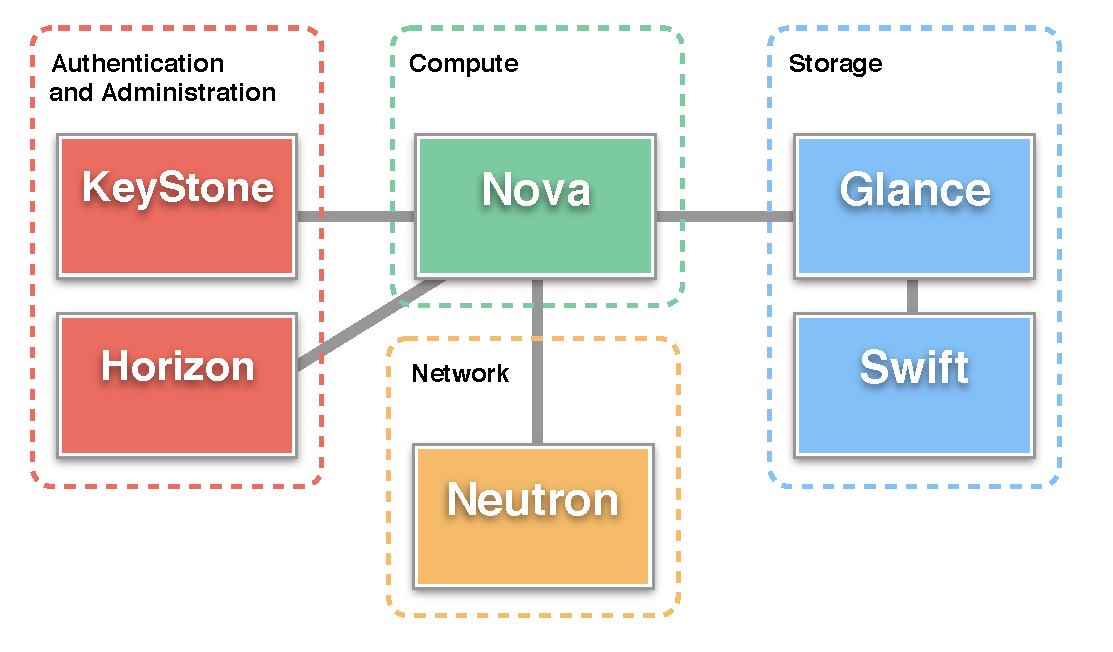
\includegraphics[width=0.75\linewidth]{Figures/openstack_architecture.pdf}
  }
	\caption{Architecture of OpenStack.}%
	\label{fig:openstack_architecture}%
	%\vspace*{-.8cm}
\end{figure*}

% - This architecture can be mapped to Moreno's architecture:
%    * Nova -> Compute manager
%    * Glance + Swift -> Storage manager
%    * Neutron -> Network manager 
%    * KeyStone, Horizon -> Authentication + Administration
% - Thus, it is possible to leverage the architecture introduced in section 3
%   over OpenStack.
Figure \ref{fig:openstack_architecture} depicts the architecture that is used by
OpenStack: it is noticeable that this can be mapped over the reference 
architecture: \emph{Nova} is very close to what is specified for the 
\emph{Compute manager} (Nova includes a static scheduler), the reunion of 
\emph{Glance} with \emph{Swift} and a DHT corresponds to the \emph{Storage 	
manager}, \emph{Neutron} exactly corresponds to the \emph{Network manager} and 
finally \emph{KeyStone} and \emph{Horizon} fits with 
\emph{Administrative tools}, \emph{Information manager} and 
\emph{Accounting/auditing}. Indeed OpenStack respects the reference 
architecture, and thus can be used to build a first prototype of the LUC-OS.

\subsection{Revisiting components for a first prototype of the LUC-OS}
\label{sub:sec:revisiting_openstack}

A typical cloud deployed with OpenStack is composed of several services (nova, 
swift, Quantum, Glance, ...) following the "shared nothing architecure" 
principle, meaning that each service is independent and thus shares no state 
with other services. In this way, inter-services collaboration is performed by 
exchanging message through an AMQP (Advanced Message Queuing Protocol) based 
bus: each service has its own queue, and it collaborates with others by sending 
messages to their queues. This offers the advantage of easily plugging 
additional components: when a default service becomes no more suitable with 
system's needs, it can be naively replaced by another custom service, as long as
the newer service consumes messages destined to the older one, and in turn 
produces messages expected by collaborators.

\subsubsection{Compute manager}
% - Nova is the angular stone of OpenStack
% - As it integrates well with OpenStack's components:
%    more LUC-OS uses NOVA -> more LUC-OS uses OpenStack's components.
% - Current version of OpenStack : only static scheduling 
%    -> replace nova-scheduler by the DVMS (dynamic scheduling).
Nova is the angular stone of OpenStack that links components together: it means
that maximizing the integration of Nova in the LUC-OS favour the reuse of 
existing components provided by OpenStack. In addition, as Nova only performs
static scheduling, we plan to replace nova-scheduler by the DVMS algorithm that 
supports dynamic scheduling.

\subsubsection{Administrative manager}
% - KeyStone and Horizon -> use the resilient fault tolerant DHT.
% - Include the VE concept.
We propose to adapt KeyStone and Horizon to make them work with the LUC-OS's
fault tolerant DHT, and to add the support of Virtual Environments.

\subsubsection{Storage manager}
% - First prototype: Test Glance and Swift.
% - if note suitable -> include recent solutions like VMTorrent 
%   (reduce network overhead).
For a first prototype, we propose to test if Glance and Swift meet LUC-OS's 
needs. If the network overhead is too significant, then we propose to leverage 
recent file storage solution like VMTorrent \cite{reich:2012}.

\subsubsection{Network manager}
% - Neutron supports plugins -> exits plugin for Open vSwitch
% - If not suitable use/develop plugins for SDN solution (Mininet or Vin).
Neutron supports plugins: it is already possible to profit the Open vSwitch 
plugin. If it appears that it is not suitable for the LUC-OS, we propose to use
(or even to develop) plugins for SDN solutions such as Mininet or Vin.



